\chapter{Series-Generation in DNA}
This chapter will deal with the general series-generation mechanisms in DNA and how to use them. Different approaches and configurations will be shown on examples to give a quick and easy insight into DNA usage.

\section{General}
The generation process uses a GraphGenerator to generate the graph and a BatchGenerator to
compile graph changes into batches. DNA offers a variety of different Graph- and BatchGenerators for different graphs and purposes. Due to the nature of dynamic graphs, metrics can either calculate their values based on initial information and additional updates or do a full recompute after each update. During generation DNA will store statistics, runtimes and computed data in series objects. A series contains one or more runs, each of which represent one separate simulation. A run is divided into several batches, which contain statistics, runtimes and metric datas, see \ref{fig:filesystem-struct}. The \textit{aggr}-directory contains aggregated data of all runs contained in the specific series. For more details on the DNA architecture and theoretical background check the DNA paper. TODO: Citation.

\begin{figure} [h]
\centering
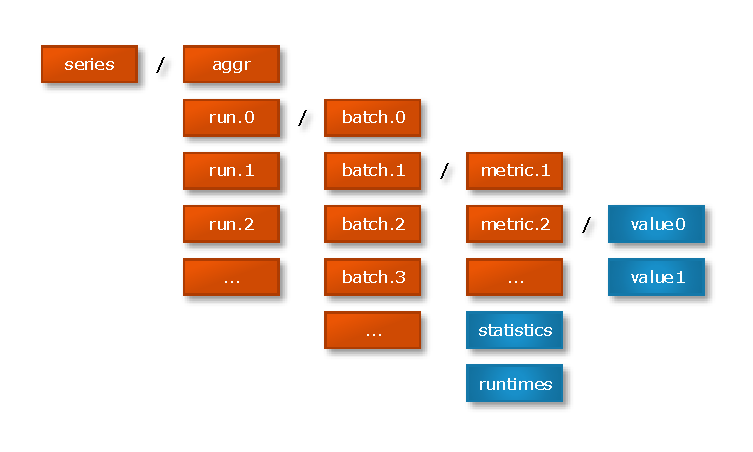
\includegraphics [scale=1.2] {images/fs-struct}
\caption{Filesystem structure for storing the results of a series.}
\label{fig:filesystem-struct}
\end{figure}

\section{Getting started}
The usual workflow is pretty simple. First one initializes a GraphGenerator, BatchGenerator and an array of metrics. Then a Series object is initialized with these inputs. The second step is the generation itself: Each Series-object has several generation-methods for different purposes. The example in \ref{code:example1} shows how one could generate a random, undirected graph with initially 100 nodes and 300 edges. With each batch 5 nodes and 20 edges are randomly being added while also 15 edges are being removed. The metrics \textit{DegreeDistributionR} (recomputed) and \textit{UndirectedClusteringCoefficientU} (updated) are chosen to be computed. 

\begin{figure} [h]
\begin{lstlisting}
public static void main(String[] args) throws AggregationException,
		IOException, MetricNotApplicableException,
		InterruptedException {
	String seriesDir = dir + "series/";

	// initialization, 100 nodes and 300 edges
	GraphGenerator gg1 = new RandomGraph(GDS.undirected, 100, 300);
	
	// 5 nodes-added, 0 nodes-removed, 20 edges-added, 15 edges-removed
	BatchGenerator bg1 = new RandomBatch(5, 0, 20, 15);
	
	// choose metrics
	Metric[] m1 = new Metric[] { new DegreeDistributionR(),
			new UndirectedClusteringCoefficientU() };

	// create series and generate it
	Series s = new Series(gg1, bg1, m1, seriesDir, "series");
	
	// generate 2 runs with 100 batches each
	SeriesData sd = s.generate(2, 100);
}
\end{lstlisting}
\caption{Simple generation example.}
\label{code:example1}
\end{figure}

\section{Auto-generated extra-values}
The DNA is able to compute additional extra values for distributions and nodevaluelists. This is enabled by default and can be finely configured in the \textit{settings.properties} configuration file. These include \textit{minimum}, \textit{maximum}, \textit{median}, \textit{average} and for certain distributions \textit{binsize} and \textit{denominator}. Consider the following example:\\

The metric \textit{DegreeDistributionR} calculates the values \textit{degreeMin}, \textit{degreeMax} aswell as the distribution \textit{DegreeDistribution}. DNA will automatically generate the additional values \textit{DegreeDistribution\textunderscore AVG}, \textit{DegreeDistribution\textunderscore MAX}, \textit{DegreeDistribution\textunderscore MED} and \textit{DegreeDistribution\textunderscore MIN}. Note: Because the \textit{DegreeDistribution} is an int-distribution it is also possible to generate an extra value \textit{DegreeDistribution\textunderscore DENOMINATOR}, however this is disabled by default.

\section{Zip-Modes}
The generation of series with lots of runs, batches and metrics can lead to a lot of single files on the filesystem. In order to reduce the amount of files aswell as the overall disk space allocation it is possible to enable zip-mode. Note that the use of zip-files leads to a higher cpu load which will result in increased runtimes. The zip-modes can either be enabled via the \textit{settings.properties} configuration file or during runtime with the config-key \textit{GENERATION\textunderscore AS\textunderscore ZIP}. Zips are disabled by default:
\begin{lstlisting}
			Config.overwrite("GENERATION_AS_ZIP", "none");
\end{lstlisting}

\subsection{Batches}
In zipped-batch mode every batch will be written and read as a single zip-file. May be enabled via the following command:
\begin{lstlisting}
			Config.overwrite("GENERATION_AS_ZIP", "batches");
\end{lstlisting}

\subsection{Runs}
In zipped-run mode every run will be written and read as a single zip-file. Note that this greatly reduces the amount of files (one for each run and an additional for the aggregation) but also greatly increases cpu load, because the zip-file has to be accessed for each read and write operation.
\begin{lstlisting}
			Config.overwrite("GENERATION_AS_ZIP", "runs");
\end{lstlisting}